\begin{savequote}[5cm]
    If in the future the laws of physics do not apply
    \qauthor{Cookie Monster}
\end{savequote}

\newcommand{\ketm}{\ket{{-}}}
\newcommand{\ketp}{\ket{{+}}}
\newcommand{\ketpm}{\ket{{\pm}}}
\newcommand{\ketz}{\ket{{0}}}
\newcommand{\keto}{\ket{{1}}}
\newcommand{\vecsigma}{\boldsymbol{\sigma}}

\chapter{Topological band structures}

We demonstrate the realization of topological band structures by exploiting the intrinsic spin-orbit coupling of dipolar interactions in combination with broken time-reversal symmetry.
The system is based on polar molecules trapped in a deep optical lattice, where the dynamics of rotational excitations follows a hopping Hamiltonian which is determined by the dipolar exchange interactions.
We find topological bands with Chern number $C=2$ on the square lattice, while a very rich structure of different topological bands appears on the honeycomb lattice.
We show that the system is robust against missing molecules.
For certain parameters we obtain flat bands, providing a promising candidate for the realization of bosonic fractional Chern insulators.

The quest for the realization of different topological states of matter marks one of the major challenges in quantum many-body physics.
A well established concept for the generation of two-dimensional topologically ordered states exhibiting anyonic excitations are flat bands characterized by a topological invariant in combination with strong interactions~\cite{Bergholtz2013,Parameswaran2013}.
The prime example is the fractional quantum Hall effect, where strong magnetic fields generate Landau levels~\cite{Nayak2008}.
Furthermore, lattice models without Landau levels have been proposed for the realization of topological bands~\cite{Haldane1988,Wang2011,Neupert2011,Wang2012a,Grushin2012,Moller2009,Barkeshli2012,Wang2011a,Sterdyniak2013,Liu2012,Yao2013,Yang2012,Cooper2013,Shi2013}.
Notably, spin-orbit coupling has emerged as an experimentally promising tool for band structures with topological invariants~\cite{Kane2005,Qi2011,Hasan2010,Tang2011}.
In this letter, we show that dipolar interactions, exhibiting intrinsic spin-orbit coupling, can be exploited for the realization of topological bands with cold polar molecules.

In cold gases experiments, the phenomenon that dipolar interactions exhibit spin-orbit coupling is at the heart of demagnetization cooling~\cite{Hensler2003,Fattori2006},
and has been identified as the driving mechanism for the Einstein-de Haas effect in Bose-Einstein condensates~\cite{Kawaguchi2006} and the pattern formation in spinor condensates~\cite{Santos2006,Vengalattore2008,Kurn2013}.
Dipolar relaxation was proposed as a mechanism to reach the quantum Hall regime by the controlled insertion of orbital angular momentum~\cite{Peter2013}.
Recently, it has been pointed out that dipolar spin-orbit coupling can be observed in band structures realized with polar molecules~\cite{Syzranov2014}.
These ideas are motivated by the experimental success in cooling and trapping polar molecules in optical lattices~\cite{Ni2008b,Yan2013}.

%In cold atomic and molecular gases experiments, the spin-orbit coupling of dipolar interactions has been utilized for demagnetization cooling~\cite{Hensler2003,Fattori2006}, and has been identified as the driving mechanism for the pattern formation in spinor condensates~\cite{Kawaguchi2006,Santos2006,Vengalattore2008,Kurn2013}.
%It has been proposed to reach the integer quantum Hall regime by the controlled insertion of orbital angular momentum by dipolar relaxation~\cite{Peter2013}.
%Recently, it has been pointed out that this spin-orbit coupling can be observed in band structures realized with polar molecules, using the dipolar exchange interaction~\cite{Syzranov2014}.
%These ideas are motivated by the experimental success in cooling polar molecules into the ground state and trapping them in optical lattices~\cite{Ni2008b,Yan2013}.


\begin{figure}[ht]
    \centering
    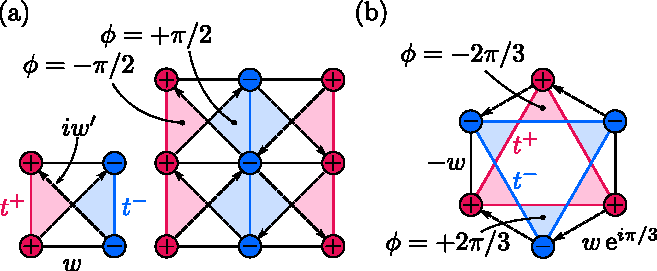
\includegraphics[width=.7\columnwidth]{topobands/fig1/fig1}

    \caption{
        \label{fig:fig1}
        (a)~Setup: Each lattice site of a two-dimensional optical lattice is occupied by a single polar molecule.
        The molecules can be excited into two different rotational states.
        Dipole-dipole interactions induce long-range tunneling links for the excitations.
        (b)~Rotational level structure of each molecule with applied electric field and additional microwave field with Rabi frequency $\Omega$ and detuning $\Delta$.
    }
\end{figure}

Here we show that a system of polar molecules gives rise to topological band structures, exploiting the spin-orbit coupling of dipolar interactions in combination with a term that breaks time-reversal symmetry.
The main idea is based on polar molecules trapped in a two-dimensional deep optical lattice with quenched tunneling between the sites.
The relevant degree of freedom of the polar molecules is given by two different rotational excitations which can be transferred between different lattice sites due to the dipolar exchange interaction.
We demonstrate that the band structure for such an excitation is characterized by a Chern number which depends on the underlying lattice structure.
In particular, we find that the system on a square lattice gives rise to Chern number $C=2$, while a rich phase diagram appears on the honeycomb lattice. % with several different Chern bands with $C$ ranging from $1$ to $4$.
Ideally, the setup is initialized with one polar molecule per lattice site, but we demonstrate that the topological properties are robust, even if nearly half of the molecules are randomly removed.
Hard-core bosons in topological bands with Chern number $C=2$ are expected to give rise to a fractional Chern insulator at $2/3$ filling~\cite{Moller2009,Wang2012a}.

The main advantages of our realization, using the spin-orbit coupling present in dipolar interactions, are its robustness and the low experimental requirements, while many alternative theoretical proposals with cold gases require strong spatially inhomogeneous laser fields with variations on the scale of one lattice constant~\cite{Liu2010,Stanescu2010,Goldman2013,Li2008,Yao2012,Yao2013,Goldman2013,Jaksch2003a}.
We point out that our proposal can also be applied to Rydberg atoms in similar setups~\cite{Barredo2014,Piotrowicz2013,Nogrette2014}.

\section{Setup}

We consider a two-dimensional system of ultracold polar molecules in a deep optical lattice with one molecule pinned at each lattice site, as shown in~\figref{fig1}a.
The remaining degree of freedom is given by the internal rotational excitations of the molecules with the Hamiltonian
\begin{align}
    H^{\text{rot}}_i &= B \vec{J}_i^2 - \vec{d}_i\cdot\vec{E}\,.
\end{align}
Here, $B$ is the rotational splitting, $\vec{J}_i$ is the angular momentum of the $i$th molecule and $\vec{d}_i$ is its dipole moment which is coupled to the applied static and microwave electric fields $\vec{E} = \vec{E}_{\text{s}} + \vec{E}_{\text{ac}}(t)$.
In the absence of external fields, the eigenstates $\ket{J,m}$ of $H^{\text{rot}}_{i}$ are conveniently labeled by the total angular momentum $J$ and its projection $m$.
% Applying a static electric field, using its direction as quantization axis, will mix states with different $J$.
Applying a static electric field mixes states with different $J$.
The projection $m$, however, can still be used to characterize the states.
In the following, we focus on the lowest state $\ketz$ with $m=0$ and the two degenerate excited states $\ketpm$ with $m = \pm 1$, see~\figref{fig1}b.

% In the following, we select two different but almost degenerate states out of the rotational manifold.
% These states might be additionally ``dressed'' by applying static and microwave electric fields.
% For concreteness, we will focus on the setup illustrated in \figref{fig1}b,c.
% Here, we select two states, called $\ketp$ and $\ketm$ below, which are adiabatically connected to the $\ket{1,1}$ and $\ket{1,{-1}}$ states.
% These states are split off from the $m=0$ state by the static electric field.

% The full system is described by $H=\sum_i H_\text{rot}^i + \frac{1}{2}\sum_{i\ne j}H_\text{dd}^{ij}$ with
% the interactions between the molecules described by the dipole-dipole interaction
% \begin{align}
%     H_{\text{dd}}^{ij} &= \frac{\kappa}{R_{ij}^3}
%     \big[{\vec{d}_i\cdot\vec{d}_j-3(\vec{d}_i\cdot\hat{\vec{R}}_{ij})(\vec{d}_j\cdot\hat{\vec{R}}_{ij})}\big].
% \end{align}
% Here, $\kappa=1/4\pi\epsilon_0$ and $\vec{R}_{ij}$ is the vector connecting the two molecules at lattice sites $i$ and $j$.
% In two dimensions, with an electric field perpendicular to the lattice, this expression reduces to
% \begin{align}
%     H_{\text{dd}}^{ij}&=\frac{\kappa}{R_{ij}^3} \Big[d^0_i d^0_j + \frac{1}{2}\big(d^+_i d^-_j -3 d^-_i d^-_j \ef{2i\phi_{ij}} + \hc\big)\Big] \label{eq:ddint}
% \end{align}
% with $d^0=d^z, d^\pm=\mp (d^x\pm i d^y)/\sqrt{2}$ the spherical components of the dipole operator
% and the polar angle $\phi_{ij}$ defined via $\smash{\hat{\vec{R}}_{ij} = (\cos \phi_{ij}, \sin \phi_{ij})^t}$.

The full system, including pairwise dipole-dipole interactions between the polar molecules, is described by $H=\sum_i H^{\text{rot}}_i + \frac{1}{2}\sum_{i\ne j}H^{\text{dd}}_{ij}$.
In the two-dimensional setup with the electric field perpendicular to the lattice, the interaction can be expressed as
\begin{align}
    H^{\text{dd}}_{ij}=\frac{\kappa}{|\vec{R}_{ij}|^3} &\Big[d^0_i d^0_j + \frac{1}{2}\big(d^+_i d^-_j + d^-_i d^+_j) \nonumber \\
                                                       &\quad - \frac{3}{2}\big(d^-_i d^-_j \ef{2i\phi_{ij}} + d^+_i d^+_j \ef{-2i\phi_{ij}}\big)\Big] \label{eq:ddint}
\end{align}
with $\kappa=1/4\pi\epsilon_0$.
Here, $\phi_{ij}$ denotes the in-plane polar angle of the vector $\vec{R}_{ij} \equiv |\vec{R}_{ij}| \cdot (\cos \phi_{ij}, \sin \phi_{ij})^t$ which connects the two molecules at lattice sites $i$ and $j$, and the operators $d^0=d^z$ and $d^\pm=\mp (d^x\pm i d^y)/\sqrt{2}$ are the spherical components of the dipole operator.
The intrinsic spin-orbit coupling is visible in the second line in Eq.~\eqref{eq:ddint}, where a change in internal angular momentum by $\pm 2$ is associated with a change in orbital angular momentum encoded in the phase factor $e^{\mp 2i \phi_{ij}}$.

For molecules with a permanent dipole moment $d$ in an optical lattice with spacing $a$, the characteristic interaction energy $V=\kappa d^2/a^3$ is much weaker than the rotational splitting $B$.
For strong electric fields, the energy separation between the states $\ketpm_i$ and $\keto_i$ is also much larger than the interaction energy.
Then the number of $\ketpm$ excitations is conserved.
This allows us to map the Hamiltonian to a bosonic model: The lowest energy state with all molecules in the $\ketz$ state is the vacuum state, while excitations of a polar molecule into the state $\ket\pm_i$ are described by hard-core boson operators $\smash{\bopd_{i,\pm} =\ket{\pm}_i\!\bra{0}_i }$.
Note that these effective bosonic particles have a spin angular momentum of $m =\pm 1$.

A crucial aspect for the generation of topological bands with a nonzero Chern number is the breaking of time-reversal symmetry.
In our setup, this is achieved by coupling the state $|+\rangle_{i}$ to the rotational state $\ket{m=2}_{i}$ with an off-resonant microwave field \footnote{The coupling of the $\ketm$ state to the third $m=0$ state can be neglected due to a large detuning from the difference in Stark shifts between $m=0$ and $m=2$}, see \figref{fig1}b.
This coupling lifts the degeneracy between the two excitations $|\pm\rangle_{i}$ and provides an energy splitting denoted by $2 \mu$.


%The system discussed so far is invariant under (pseudo-spin) time-reversal represented by $\mathcal{T}=\sigma_x K$, with $K$ being complex conjugation.
%A necessary requirement for bands with nonzero Chern number is the opening of bandgaps at the $\Gamma$ and $K$ point and the breaking of $\mathcal{T}$-symmetry~\cite{Haldane1988}.
%We achieve this by using a circularly polarized microwave to couple the $\ketp$ state off-resonantly to the lowest $m=2$ state~\footnote{The coupling of the $\ketm$ state to the third $m=0$ state can be neglected due to a large detuning from the difference in Stark shifts between $m=0$ and $m=2$}, see~\figref{fig1}(c).
%This has two effects for the model in~\eqref{eq:hrealspace}.
%First, the AC Stark shift introduces an energy offset for the dressed $\ketp$ state (relative to the $\ketm$ state).
%Note that, in addition, this shift can be independently controlled via magnetic fields~\cite{Ospelkaus2010,Yan2013}.
%Second, the tunneling strength $t^+$ of the $\ketp$ particles now differs from the one of the $\ketm$ particles ($t^-$).
%In turn, the model is now described by a modified vector

\section{Bosonic model and band structure}

The dipole-dipole interaction gives rise to an effective hopping Hamiltonian for the bosonic particles due to the dipolar exchange terms:
$d^+_id^-_j$, for example, leads to a (long-range) tunneling $\bopd_{i,+}\bop_{j,+}$ for the ${+}$-bosons while the term $d^-_i d^-_j \ef{2i\phi_{i j}}$ generates spin-flip tunneling processes $\bopd_{i,-}\bop_{j,+} \ef{2i\phi_{ij}}$ with a phase that depends on the direction of tunneling.
For the study of the single particle band structure we can drop the term proportional to $d^0 d^0$ which describes a static dipolar interaction between the bosons.
The interaction Hamiltonian reduces to
\begin{align}
    H^{\text{dd}} = \sum_{i\ne j}
    \frac{a^3}{|\vec{R}_{ij}|^3}\;
    \psiopd_i\!
    \begingroup
        \renewcommand*{\arraystretch}{1.2}
        \begin{pmatrix}
            -t^+ & w \ef{-2i\phi_{ij}} \\
            w \ef{2i\phi_{ij}} & -t^-
        \end{pmatrix}
    \endgroup\!
    \psiop_j \,,
    \label{eq:hrealspace}
\end{align}
where we use the spinor notation $\psiopd_j = \big( \bopd_{j,+} , \bopd_{j,-} \big)$.
% The precise form of the hopping rates $t^+$, $t^-$, and $w$ depends on the microscopic parameters and the detailed expressions are presented in the supplementary material.
% The energy scale is given by the characteristic energy of the dipole-dipole interaction $V$.
The energy scale of the hopping rates $t^+$, $t^-$, and $w$ is given by $V$. The precise form depends on the microscopic parameters and is detailed in the supplementary material.
Note that $t^{+} = t^{-}$ without the applied microwave.
In momentum space with $\psiop_{\veck}=\frac{1}{\sqrt{N_s}}\sum_{j} \psiop_{j}\ef{i\veck\vec{R}_j}$, including the internal energy $H_{i}^{\text{rot}}$ of the excitations $|\pm\rangle_{i}$, the Hamiltonian reduces to
\begin{align}
    H &= \sum_{\veck} \psiopd_{\veck} \big({n^{0\vphantom\dagger}_{\veck} \: \mathds{1} + \vec{n}^{\vphantom \dagger}_{\veck}\cdot\vecsigma}\big) \psiop_{\veck}
    \label{eq:hkspace}
\end{align}
where $\vecsigma$ denotes the vector of Pauli matrices.
We introduce the dipolar dispersion relation~\cite{Peter2012b,Syzranov2014}
\begin{align}
    \epsilon^m_{\veck} = \sum_{j\ne 0} \frac{a^3}{|\vec{R}_j|^3}\ef{i\veck \vec{R}_j + i m \phi_{j}}, % = \big(\epsilon^{-m}_{\veck}\big)^*
\end{align}
which determines the spin-independent hopping $n^0_{\veck} = -\bar{t}\, \epsilon^0_{\veck}$, as well as the spin-orbit term characterized by the vector
\begin{align}
    \vec{n}^{\vphantom 0}_{\veck} = \begin{pmatrix}
        w \Re \epsilon^2_{\veck} \\
        w \Im \epsilon^2_{\veck} \\
        \mu + t\, \epsilon^0_{\veck}
    \end{pmatrix}
\end{align}
with ${\bar t} =( t^{+}+t^{-})/2$, $t = (t^--t^+)/2 > 0$, and the energy splitting $\mu$. % \mu = (E_+ - E_-)/2 is actually just half the energy splitting...
The precise determination of $\epsilon^m_{\veck}$ can be achieved by an Ewald summation technique providing a non-analytic low momentum behavior
$\epsilon^0_{\veck} \approx \epsilon^0_{\Gamma} - 2\pi |\veck|a$ and
$\epsilon^2_{\veck} \approx -\frac{2\pi}{3} |\veck|a \ef{2i \varphi}$.
Here, $\epsilon^0_{\Gamma} \approx 9.03$ and $\varphi$ is defined by $\hat{\veck}=(\cos \varphi, \sin \varphi)^t$.
% and $\epsilon^0_{\Gamma} = 4\zeta(\sfrac{3}{2})\beta(\sfrac{3}{2})\approx 9.03$ can be expressed with the Riemann $\zeta$-function and the Dirichlet $\beta$-function~\cite{Glasser1973}.

\begin{figure}[ht]
    \centering
    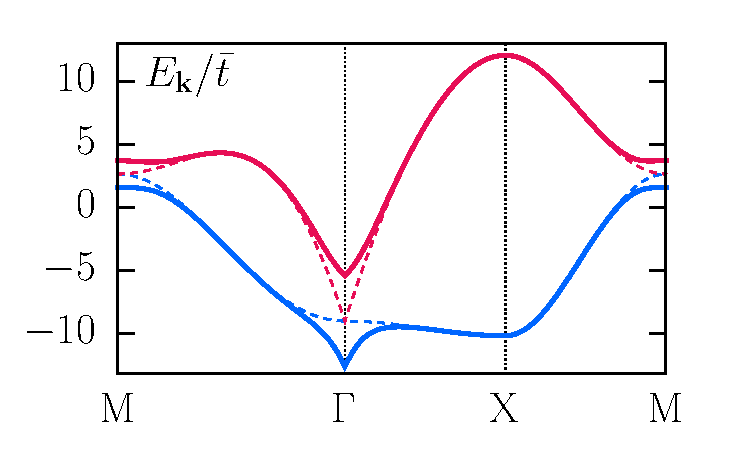
\includegraphics[width=.38\columnwidth]{topobands/fig2/fig2a}
    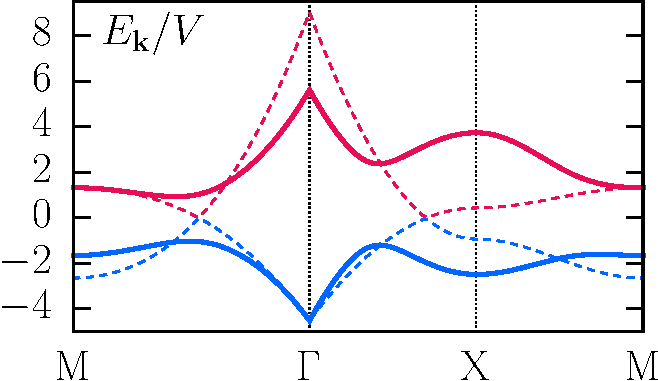
\includegraphics[width=.38\columnwidth]{topobands/fig2/fig2b}

    \caption{
        \label{fig:fig2}
        (a) Dispersion relation for the $\ketp$ and $\ketm$ states on the square lattice.
        The dashed line shows the time-reversal invariant point $t=\mu=0$ with band touching at the $\Gamma$ and $\text{M}$ point.
        % The band minima are located at the two $\text{X}$ points $(\pi/a,0)$ and $(0, \pi/a)$.
        The solid line shows the gapped topological bands in the time-reversal-broken system for $w/\bar{t}=3, \mu=0$ and $t/\bar{t}=0.4$.
        % For $t/\bar{t}\gtrsim 0.13$, the band minimum is at the $\Gamma$ point.
        (b) Dispersion relation for the $\ketp$ and $\keto$ states for electric field angles $\Theta_0=0$ (dashed) and $\Theta_0=\pi/4$ (solid), respectively.
        The latter has a lower band with flatness $f\approx 1$.
        % Note: The two '\text{X}' points in the Brillouin zone (pi,0) and (0,pi) are not equivalent as the electric field breaks the x/y symmetry.
    }
\end{figure}

In the presence of time-reversal symmetry, represented by $\mathcal{T}=\sigma_x \mathcal{K}$ with $\mathcal{K}$ being complex conjugation, the system reduces to the one discussed in ref.~\cite{Syzranov2014}.
At the $\mathcal{T}$-invariant point, i.e. $t=\mu=0$, the two energy bands of the system exhibit a band touching at the high-symmetry points $\Gamma=(0,0)$ and $\text{M}=(\pi/a, \pi/a)$ where $\epsilon^2_\veck$ vanishes, see \figref{fig2}a.
%take the from
%\begin{align}
  %  E_\pm(\veck)=n^0_{\veck} \pm |\vec{n}_{\veck}|= \bar{t} \bb{-\epsilon^0_\veck \pm 3 |\epsilon^2_{\veck}|}.
%\end{align}
%The band gap closes at the two high-symmetry points $\Gamma=(0,0)$ and $\text{M}=(\pi/a, \pi/a)$ where $\epsilon^2_\veck$ vanishes.
% Both points are band touchings, where the one at the $\Gamma$ point becomes linear as a consequence of the dipolar dispersion.\\
The touching at the $\Gamma$ point is linear due to the low-momentum behavior of $\epsilon^m_\veck$.
%The lower band at the $\Gamma$ point is flat due to the exact cancellation of the linear terms.
% Note that stretching the square lattice into a rectangular lattice splits each of the band touching points into two Dirac points.
Note that each of the touching points splits into two Dirac points if the square lattice is stretched into a rectangular lattice.

Breaking of time-reversal symmetry by the microwave field leads to an opening of a gap between the two bands.
The dispersion relation is given by
\begin{align}
    E_\pm(\veck)=- \bar{t}\, \epsilon^0_\veck \pm \sqrt{w^2 \big|\epsilon^2_{\veck}\big|^2+\big(\mu+t\, \epsilon^0_{\veck}\big)^2}
\end{align}
and shown in \figref{fig2}a.
It is gapped whenever the vector $\vec{n}_{\veck}\ne 0$.
The first two components can only vanish at the $\Gamma$ or $\text{M}$ point.
% Consequently, the vanishing of the third component at these points yields a necessary and sufficient condition for a gap closing.
Consequently, the gap closes iff the third component is zero at one of these two points, that is for
% We find the two transition points
\begin{align} % we could replace t -> -t to have eps_Gamma and eps_K here...? (But: t would be negative)
    \mu/t &= -\epsilon^0_{\Gamma} \approx -9.03, \nonumber\\
    \mu/t &= -\epsilon^0_\text{M} = \Big(1-1/\sqrt{2}\Big)\epsilon_{\Gamma}^0 \approx +2.65.
\end{align}
In the gapped system, the Chern number~\cite{Hasan2010,Qi2011} can be calculated as the winding number of the normalized vector $\hat{\vec{n}}_\veck = \vec{n}_\veck/|\vec{n}_\veck|$ via
\footnote{We remark that we need to truncate the summation in the expression for $\epsilon^m_{\veck}$ to perform the calculation of the Chern number.
We can check, however, that the remaining terms are not strong enough to close a gap.
Conversely, note that the cutoff radius has to be larger than $\sqrt{2}a$, as the next-to-nearest neighbor terms are crucial for the $C=2$ phase and may not be neglected.}
\begin{align}
    C &= \frac{1}{4\pi}\int_{\text{BZ}}\!\mathrm{d}{^2\veck}\, ( \partial_{k_x} \hat{\vec{n}}_{\veck} \times \partial_{k_y} \hat{\vec{n}}_{\veck} ) \cdot \hat{\vec{n}}_{\veck} \, . \label{eq:chern}
\end{align}
We find that the Chern number of the lower band is $C=2$ for $-\epsilon^0_{\Gamma} < \mu/t < -\epsilon^0_\text{M}$, and zero outside this range.
% Note that the non-trivial topology is purely a consequence of the spin-orbit coupling by dipolar interaction in combination with time-reversal symmetry breaking.
Note that the non-trivial topology solely results from dipolar spin-orbit coupling and time-reversal symmetry breaking.



\begin{figure}[ht]
    \centering
    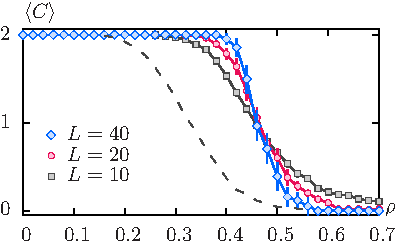
\includegraphics[width=.43\columnwidth]{topobands/fig3/fig3a}
    \hspace{0.1cm}
    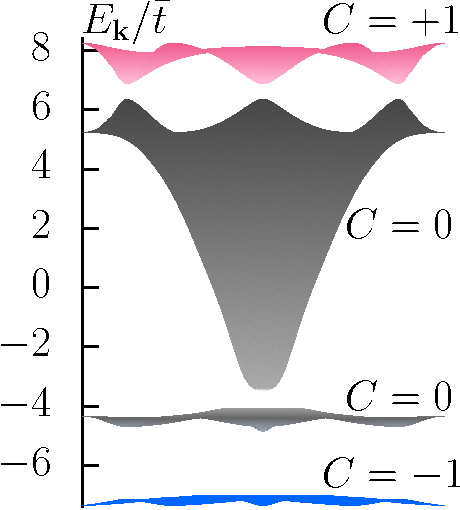
\includegraphics[width=.22\columnwidth]{topobands/fig3/fig3b}
    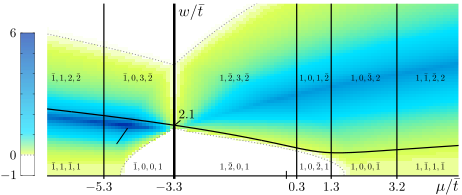
\includegraphics[width=.7\columnwidth]{topobands/fig3/fig3c}

    \caption{
        \label{fig:fig3}
        (a)~Sample-averaged Chern number $\langle C \rangle$ in the disordered system for increasing density $\rho$ of defects.
        A single realization either yields $C=2$ or $C=0$.
        Bars indicate two standard errors.
        The results are shown for square lattices of size $L \times L$ with $L=10, 20, 40$.
        % and a cutoff radius for the interaction $R_c \lesssim L/2$ slightly smaller than half the system size to avoid self-interaction.
        The long-range tunneling stabilizes the topological phase for defect densities $\rho \lesssim 0.45$.
        % As a comparison, the dashed line shows the results for a $10 \times 10$ grid with tunneling only included up to the next-to-nearest neighbor, leading to a significant destabilization.
        (b)~Two-dimensional projection of the dispersion relation in the honeycomb lattice for $t/\bar{t}=0.54, w/\bar{t}=1.97$ and $\mu/\bar{t}=-4.54$.
        The lowest band has a flatness ratio of $f\approx 6.4$ and a Chern number of $C=-1$.
        (c)~Topological phase diagram in the honeycomb lattice for $t/\bar{t}=0.54$.
        The labels give the Chern numbers of the four bands (bar indicates negative number) from bottom to top while the solid lines correspond to touching points between two bands.
        The color indicates the flatness $f$ of the lowest band.
        The arrow shows the parameters of the flat-band model in~(b).
    }
\end{figure}


% The main quest is then to optimize the setup in order to optimize the flatness of topological bands.
The challenge is to find a specific setup that optimizes the flatness of the topological bands.
This can be achieved either by focusing on different lattice structures (see honeycomb lattice below and \figref{fig3}b) or by an alternative choice for the two excitations.
The latter is less intuitive when trying to understand the spin-orbit coupling, but gives rise to significantly flatter bands: Instead of considering $\ketp$ and $\ketm$, we choose a model including the $\ketp$ and $\keto$ states.
This is possible for weak electric fields, if the $\ketm$ state is shifted by a microwave field, or by exploiting the coupling between the nuclear spins of the polar molecules and the rotational degree of freedom~\cite{Ospelkaus2010,Yan2013}.
This model intrinsically breaks time-reversal symmetry and has the advantage that the $\ketp$ and $\keto$ states have different signs for the tunneling strength, making the $\mathcal{T}$-breaking parameter $t=(t^+-t^1)/2$ large compared to $\bar{t}=(t^++t^1)/2$. % in fact, we know that t/tbar = 3t^+/(-t^+) = -3
For an electric field direction perpendicular to the lattice, this system is gapless.
Opening the gap is achieved by rotating the electric field away from the $z$-axis by an angle $\Theta$.
The dispersion relation for $\Theta=0$ and $\pi/4$ is shown in~\figref{fig2}b.
The lower band has a flatness ratio of $f = \text{bandgap}/\text{bandwidth} \approx 1$.
%While not being as good as the ratios achieved in related proposals~\cite{Yao2012,Yao2013,Neupert2011,Trescher2012,Wang2011a,Yang2012}, we stress that only a single parameter $\Theta$ is `fine-tuned' here. The values of $t^+, t^1$ and $w$ for weak fields are fixed by the dipole-dipole interaction.


Topological band structures are classified by considering equivalence classes of models that can be continuously deformed into each other without closing the energy gap~\cite{Hasan2010}.
% In particular, the Chern number of a single band can only change if it touches another band.
Using this idea, we can demonstrate that our model with $C=2$ is adiabatically equivalent to a system of two uncoupled copies of a $C=1$ layer (see supplementary material for details).
% The single layer system has some interesting properties, as it can be described by a staggered magnetic flux pattern.
The resulting single layer model can be described by a staggered flux pattern and is reminiscent of the famous Haldane model~\cite{Haldane1988}, adapted to the square lattice~\cite{Goldman2013,Li2008,Liu2010,Liu2011,Stanescu2010,Wang2011,Wang2014,Yao2012,Yao2013}.
It is rather remarkable that uniform dipole-dipole interactions give rise to a model usually requiring strong modulations on the order of the lattice spacing.
%Using a site-dependent microwave dressing, it has been shown that a model similar to our single-layer system can be realized, giving rise to a $\nu=1/2$ fractional Chern insulating phase~\cite{Yao2012,Yao2013}.



\section{Influence of disorder}

An experimental initialization with a perfectly uniform filling of one molecule per site is challenging.
Consequently, we analyze the stability of the topological band structure for random samples with a nonzero probability $\rho$ for an empty lattice site.
The determination of the Chern number for the disordered system follows ideas from refs.~\cite{Niu1985,Avron1985}.
We start with a finite geometry of $L \times L$ lattice sites and twisted boundary conditions
% \begin{align}
%     \psi(x + L, y) &= \ef{i\theta_x}\psi(x, y), \\
%     \psi(x, y + L) &= \ef{i\theta_y}\psi(x, y).
% \end{align}
$\psi(x + L, y) = \ef{i\theta_x}\psi(x, y)$ and $\psi(x, y + L) = \ef{i\theta_y}\psi(x, y)$ for the single particle wave function.
Next, we randomly remove $\rho L^2$ lattice sites (dipoles).
We are interested in the Chern number of the lower `band', composed of the lowest $N_l=L^2 (1-\rho)$ states (there are $2N_l$ states in total).
To this end, we pretend to have a free fermionic system at half filling whose many-body ground state $\Psi=\Psi(\theta_x, \theta_y)$ is given by the Slater determinant of the lowest $N_l$ states.
Then, the Chern number can be calculated as
\begin{align}
    C &= \frac{1}{2\pi}\iint\!\mathrm{d}\theta_x \mathrm{d}\theta_y \, F(\theta_x, \theta_y), \label{eq:manybodychern}
\end{align}
where $F(\theta_x,\theta_y)=\smash{\Im\!\big({\big\langle\frac{\partial \Psi}{\partial \theta_y}\big|\frac{\partial \Psi}{\partial \theta_x}\big\rangle - \big\langle\frac{\partial \Psi}{\partial \theta_x}\big|\frac{\partial \Psi}{\partial \theta_y}\big\rangle}\big)}$ is the many-body Berry curvature depending on the boundary condition twists.
Note that Eq.~\eqref{eq:manybodychern} reduces to~Eq.~\eqref{eq:chern} in the translationally invariant case.
For the numerical computations, we use a discretized version~\cite{Fukui2005}.
The results for the disordered system are summarized in~\figref{fig3}a.
We find that the long-range tunneling stabilizes the topological phase for defect densities $\rho\lesssim 0.45$.
% We find that the topological phase is robust for defect densities $\rho\lesssim 0.45$.
% The long-range tunneling ${\sim}|\vec{R}|^{-3}$ is found to significantly enhance the stability compared to a model with artificial truncation at the next-to-nearest neighbor level.
% parameters for the disorder calculations: $\bar{t}=\mu=0, w=3t$.

\section{Other lattices}

\subsection{Honeycomb lattice:}
Returning to the simple setup in \figref{fig1}b, the influence of the lattice geometry can be exemplified by going to the honeycomb lattice.
Due to the two distinct sublattices, we generally obtain four bands in the presence of broken time-reversal symmetry.
Depending on the microscopic parameters, the bands exhibit a rich topological structure, characterized by their Chern numbers.
Note that the Chern numbers are calculated with a numerical method similar to the one for the disordered system.
In \figref{fig3}c, we show a two-dimensional cut through the topological phase diagram, spanned by the parameters $t/\bar{t}, w/\bar{t}$ and $\mu/\bar{t}$.
We find a multitude of different topological phases with large areas of flatness $f > 0$ for the lowest band.
A flatness $f < 0$ indicates that the maximum of the lowest band is higher than the minimum of the second band.
In contrast to the square lattice, an energy splitting $\mu \ne 0$ is sufficient for a nonzero Chern number; $t\ne 0$ is not necessarily needed.
\figref{fig3}b shows the dispersion relation with a lowest band of flatness $f\approx 6.4$ and a Chern number $C=-1$.

% The relation to the bilayer system allows us to explain the behavior of this model on different 2D lattices.
% Assigning ${+}$ and ${-}$ orbitals to the two distinct sublattices yields a single layer with a Chern number of $C=1$.
% In contrast to the square lattice, however, the Brillouin zone of a single layer is the same as for the full (double layer) system with both orbitals at each site.
% As a result, the lowest (of four) bands in the honeycomb lattice can have a Chern number of $C=1$~\footnote{The inter-layer coupling in the bilayer honeycomb system is crucial to open a gap.}.

\begin{figure}[ht]
    \centering
    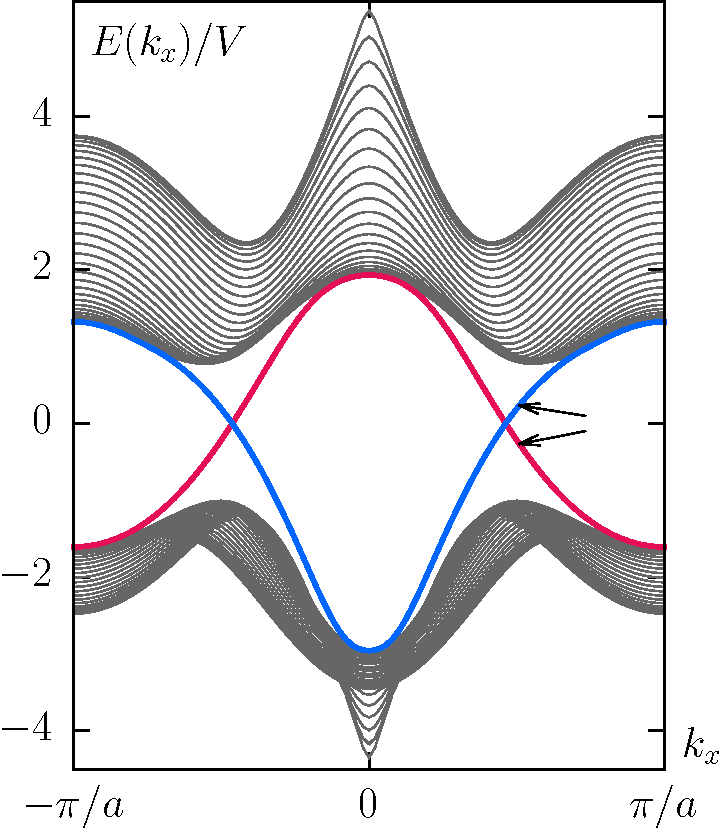
\includegraphics[width=.504\columnwidth]{topobands/fig4/fig4a}
    \begin{minipage}[b]{.482\columnwidth}
        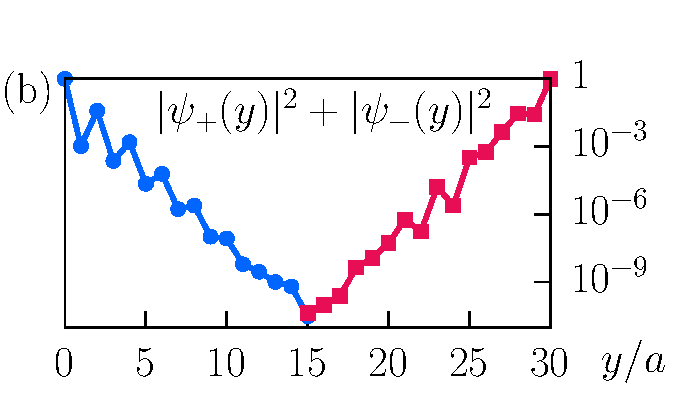
\includegraphics[width=.95\columnwidth]{topobands/fig4/fig4b} \\
        \vspace{2mm}
        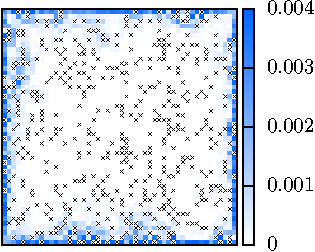
\includegraphics[width=.95\columnwidth]{topobands/fig4/fig4c}
    \end{minipage}

    \caption{
        \label{fig:fig4}
        (a)~Dispersion relation for the $\ketp$ and $\keto$ states on a cylindrical square lattice geometry with infinite extent in $x$ direction and $31$ sites in $y$ direction.
        Four edge states cross the bandgap in the $C=2$ phase (two for each edge).
        (b)~Exponentially decaying amplitude of the two edge states corresponding to the points shown in the spectrum.
        (c)~Edge state amplitude $|\psi_+(x,y)|^2 + |\psi_-(x,y)|^2$ on a finite $50 \times 50$ square lattice with a fraction $\rho=0.2$ of the molecules removed (missing sites are indicated by crosses).
    }
\end{figure}

\section{Detection}
One way to detect the topological band structure experimentally is to create a local excitation close to the edge of the system.
In \figref{fig4} we show the edge states in the $C=2$ phase on the square lattice.
The states are exponentially localized on the boundary of the system and the propagation of a single excitation along the edge can be used as an indication of the topological nature of the bands~\cite{Hafezi2013}.
In \figref{fig4}c, we show the robustness of the edge states against missing molecules.
The edge state is also visible in a spectroscopic analysis, as a single mode between the broad continuum of the two bands (see~\figref{fig4}a).

\section{Many-body system}
Finally, the most spectacular evidence of the topological nature would be the appearance of fractional Chern insulators in the many-body system at a fixed density of excitations.
Here, the hard-core constraint naturally provides a strong on-site interaction for the bosons.
In addition, the remaining static dipolar interactions are a tunable knob to control the interaction strength.
The most promising candidate for a bosonic fractional Chern insulator in a band with $C=2$ appears for a filling of $\nu = 2/3$, as suggested by numerical calculations~\cite{Moller2009,Wang2012a}.
